\documentclass[../../main.tex]{subfiles}

\begin{document}
    

\section{TCP/IP}
\subsection{Introduction}
Before treating such topic we must briefly discuss the behaviour of the
TCP/IP (\textbf{Internet protocol suit}) communications.

\subsubsection{IP (Internet Protocol)} IP is at the basis of internet
communication. The protocol exploits the principle of encapsulation, sending
packets composed by a \emph{header} which contains information such as the
\textbf{destination address} and \textbf{source address} and a
\emph{payload} which represents the actual data to be transmitted.
Since physical channels usually have a limited \emph{MTU}\footnote{Maximum
Transmission Unit}, then the data is usually fragmented in smaller chunks,
wrapped into an header and only then transmitted.

\subsubsection{TCP (Transmission Control protocol)} TCP is a protocol used for
reliable (little information loss), ordered, error-checked data transmission
between a machine hosting the data (\textbf{Server}) and another requiring
such data (\textbf{Client}). It is performed previous a three-way handshake
which estabilishes a connection between server and client, thus preparing a
reliable communication channel.

\subsubsection{UDP (User Datagram Protocol)} Contrary to TCP, UDP is less
reliable but faster.
It broadcasts the data in an unordered and uncontrolled way to the receiver. 
There is no need to estabilishing a connection in order to implement such
protocol.

\begin{figure*}[h]
    \centering
    \begin{subfigure}{.45\textwidth}
        \centering
        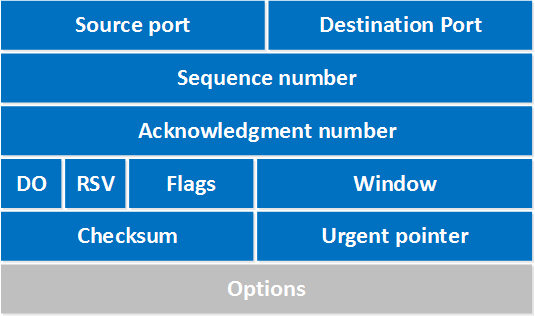
\includegraphics[width=.45\linewidth]{tcp_header.png}
        \caption{Structure of TCP packet}
    \end{subfigure}%
    ~
    \begin{subfigure}{.45\textwidth}
        \centering
        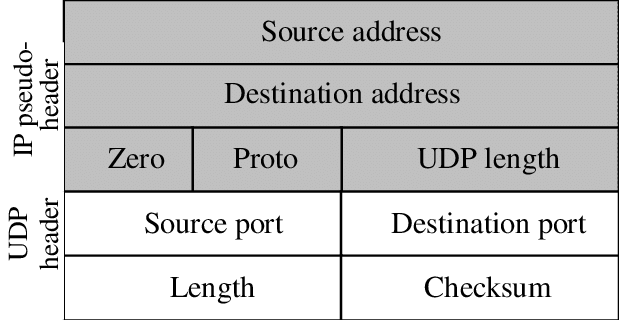
\includegraphics[width=.45\linewidth]{udp_header.png}
        \caption{Structure of UDP packet}
    \end{subfigure}
\end{figure*}

\subsection{Exploits and protection tools}

As you could notice from the previous figures, the first part of the header
is the same. This is because it is part of the IP protocol itself.
In the second part of each header we find different types of metadata which
are specific for each protocol. Generally the metadat contained in the
header is redundant for the transmission of the message itself and this 
redundancy may become a target for a \emph{stego-algorithm}\footnote{an
algorithm used for steganography} which starting from a \emph{cover-network
packet sequence}\footnote{a sequence of packets which will be transmitted
over the network acting as a cover for the hidden messace} and a
\emph{covert message}, can generate a sequence of packets(each one embedding
a portion of the covered message) which will be sent over the network.

This procedure is not a \emph{risk-free} approach for the attacker who
wishes to send the \emph{cover-network packet sequence}, since it is
possible that the data will be currupted during transmission or there could
be losses using non-reliable transport protocols(UDP).
Other criticalities of such method stay in the fact that the sequence of
packets will most likely traverse multiple nodes in the network before
reaching the target, and the message may be detected by these nodes.

The defense against Steganography in TCP/IP communication consists in 
series of standards which are implemented by the devices on the internet and
that we will illustrate through some examples.


\subsubsection{Tos (Type of service)}
Tos are a field in the TCP header which
are nowdays rarely used. This could open doors to a steganographic attack if
modern operating systems did not set them to zero by default.
A warden monitoring the channel could immediately signal an error.

\subsubsection{IP ID} IP ID is a field in the Internet Protocol which is used to
assist the receiver in reassemblying the fragmented packets.
This field consist of randomly unique numbers representing a packet.
It is possible to insert other types of information in this field by simply
conform to the uniqueness constraint.
Since in many cases the numbers used for the IP ID are not random, by
knowing the charachteristics of the sender it is possible to detect an
infiltration.

\subsubsection{IP Fragment Offset} IP Fragment Offeset is an offset which is
present in the IP header which helps the receiver to reconstruct the sequence of
bits from the fragmented sequence.
Modulating the size of the fragments changes the offset field in the header
and thus a message could be sent.
The protection against this method is simply checking the size of the
packets relative to the MTU and so even in this case a warden can easily
detect an error.

\subsubsection{TCP sequence number} The TCP sequence number is a field in the
TCP header which stores the randomly chosen position(for security reasons) of
the first byte to be transmitted through the channel. The steganographic method
consists in replacing this field with the data to be sent.
Being random it is more difficult to spot a breach in the channel.
In this case the usage of a \emph{SVM}\footnote{Support Vector Machine}, a
machine learning tool able to identify patterns inside the data transmitted
could come into hand.
However an error could be detected even simply by checking the presence of
repetitions in the stream(not admitted by design). 

\subsubsection{Timestamp modulation} Timestamp modulation is another technique
of steganography which operate by modifing the \emph{LSB} of the timestamp of a
TCP packet in order to represent a '1'.
The covert message is thus embedded into the data stream.
Since the TCP Timestamp support is not universal, machines not supporting
such feature may detect the hidden message.


\subsection{Detection of TCP/IP steganography}

Each operating system exhibits well defined characteristics in generated
TCP/IP fields. These can be used to identify any anomalies that may indicate 
the use of steganography. For this purpose, a suite of tests which may be
applied to \emph{network traces}\footnote{function that performs network
analysis on a geometric network} are defined and they are used to identify
whether the results are consistent with the operating systems believed to be
installed on the source host.
Diffreent methods of covert channel detection are used, employing IP ID 
characteristics, TCP ISN characteristics and explicit steganography
detection.

\subsubsection{IP ID characteristics}
IP ID characteristics are the features identifying the IP
address, a unique address that identifies a device on the internet or local
network. They are employed by the following methods.
\emph{Sequential Global IP ID} implies the usage of a global counter for the
IP ID. 
To detect this strategy one has to look if connections to different hosts
have sequentially increasing IP IDs.
\emph{Sequential Per-host IP ID} is characterized by the usage of a per-host
counter for packets. If it apperas to be fragmented, the warden can test
whether connections to different hosts use apparently unrelated IP IDs;
however connections to the same host have a sequentially increasing IP ID.
\emph{IP ID MSB Toggle} represents the case where the operating system
system toggles the most significant bit of the IP ID every rekey interval,
so that the warden can examine the MSB to check if it matches this pattern.
\emph{IP ID Permutation} strategy presence can be discarded by the warden if
there are duplicates, since within a rekey interval the IP ID is
non-repeating.

\subsubsection{Explicit steganography detection}
Explicit steganography detection can be employed by several
methods.
\emph{Nushu Criptography} is a strategy applied by Nushu, which encrypts
data before including it in the ISN field, resulting in a distribution which
differs form the one that is normally generated by Linux; therefore, it can
be detected. 
\emph{TCP Timestamp} strategy involves the execution of a randomness test.
In particular, if a low bandwidth TCP connection is being used to leak
information, this test can be applied to the LSBs of the timestamps in the
TCP packets. If an excessive presence of randomness is detected in the LSBs,
it can be deduced that a steganographic covert channel is in use.
There are also other features which may indicate the usage of steganography:
\emph{unsual flags}, \emph{excessive fragmentation}, use of \emph{IP
options}, \emph{unexpected TCP options} and \emph{excessive re-ordering}.


\end{document}